\documentclass[../projekt.tex]{subfiles}
\begin{document}


\chapter{Uživatelská příručka}

Tato aplikace slouží k demonstraci Kargerova algoritmu. 

\section{Ovládání aplikace}


	\begin{figure}[ht]
    	\begin{center}
  			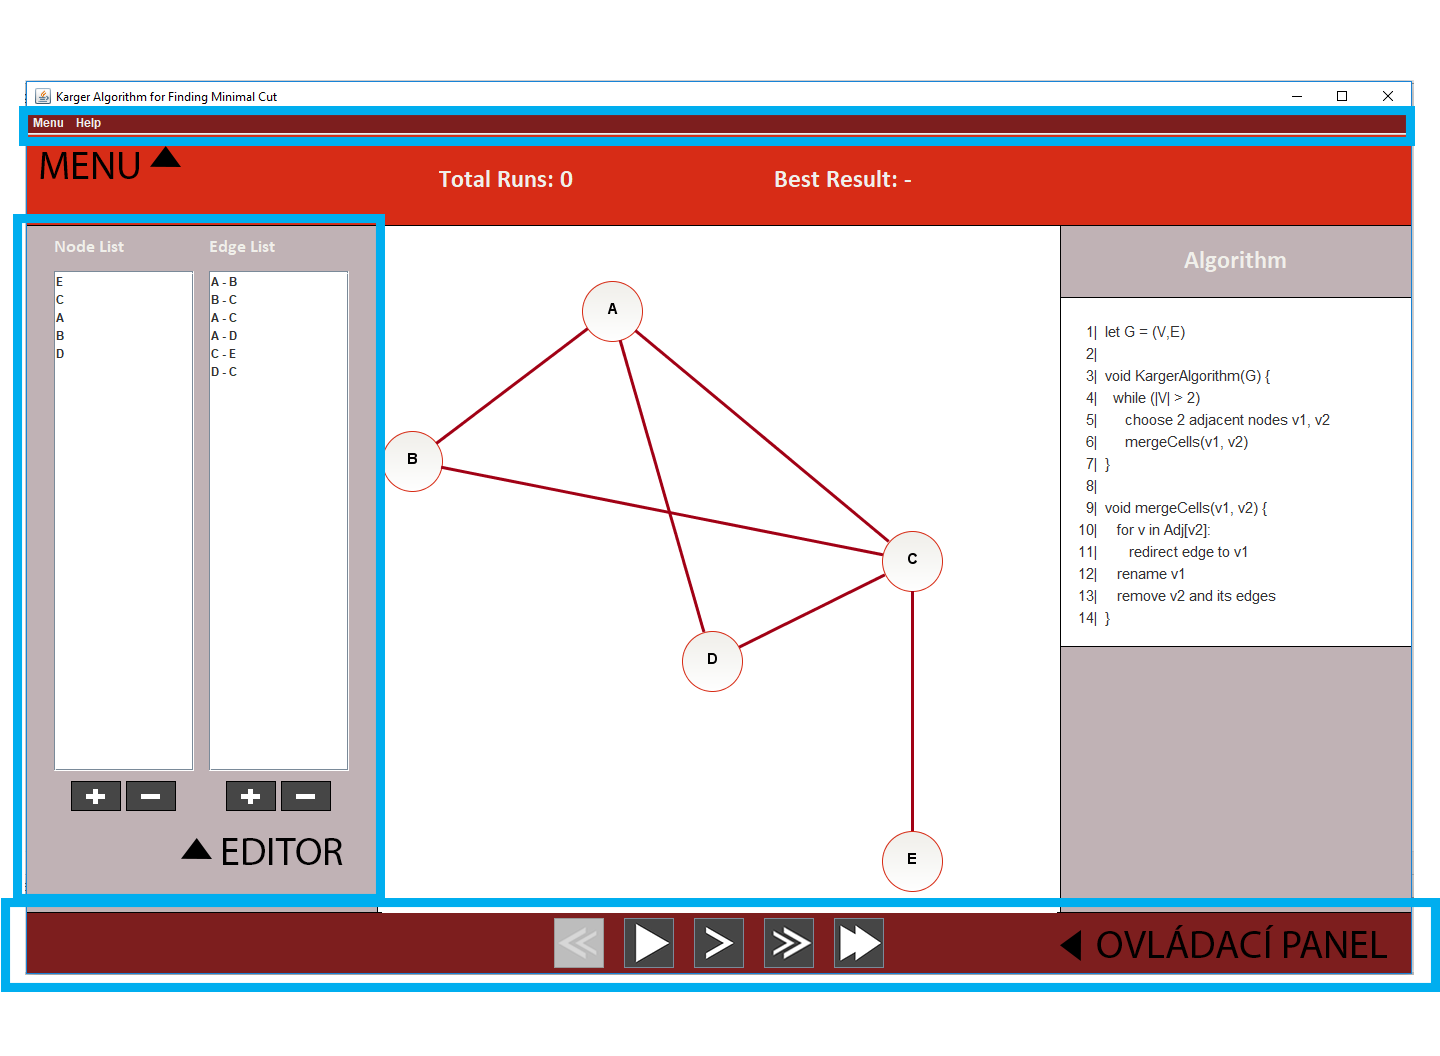
\includegraphics[scale=0.36]{obrazky-figures/ovladani.png}
  			\caption{Rozhraní ovládání aplikace.}
  		\end{center}
	\end{figure}
	
Aplikaci lze ovládat pomocí:
	
\begin{itemize}
	\item MENU - Práce se souborem, nápověda.
	\item EDITORU - Úprava grafu.
	\item OVLÁDACÍHO PANELU - Aplikace algoritmu na graf.
\end{itemize}




\subsection{Menu}

\begin{itemize}
    \item 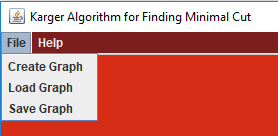
\includegraphics[height=10em]{obrazky-figures/file.png} \\Možnosti práce se souborem: \\ - vytvoření nového grafu \\ - načtení uloženého grafu ve formátu XML \\ - uložení grafu ve formátu XML
    \item 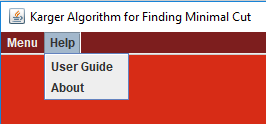
\includegraphics[height=10em]{obrazky-figures/help.png} \\Možnosti nápovědy: \\ - uživatelská příručka \\ - aplikaci
\end{itemize}



\subsection{Editor}

Editor obsahuje seznam uzlů (Node list) a seznam hran (Edge list). Ke každému z těchto seznamů jsou přidružena dvě tlačítka: 

\begin{itemize}
    \item 
\includegraphics[height=1.3em]{obrazky-figures/addButton.png} - Vložení uzlu/hrany do grafy
    \item 
\includegraphics[height=1.3em]{obrazky-figures/removeButton.png} - Odebrání uzlu/hrany z grafu
\end{itemize}



\subsection{Ovládací panel}

\begin{itemize}
    \item 
\includegraphics[height=1.3em]{obrazky-figures/resetSmall.png} - Reset předchozích kroků.
    \item 
\includegraphics[height=1.3em]{obrazky-figures/playSmall.png} - Krok vpřed.
    \item 
\includegraphics[height=1.3em]{obrazky-figures/nextStepSmall.png} - Dokončení jednoho běhu algoritmu.
    \item 
\includegraphics[height=1.3em]{obrazky-figures/finishSmall.png} - Úplně dokončení algoritmu, dojde k zobrazení výsledků.
    \item 
\includegraphics[height=1.3em]{obrazky-figures/manualSteps.png} - Krokování algoritmu v pravém panelu a zobrazování změn na grafu.
\end{itemize}

\end{document}